% print no page number
\thispagestyle{empty}

\chapter{Procedural Content Generation}

Το αντικείμενο του Procedural Content Generation (PCG) όπως ορίζεται στο [1] είναι η \textit{Δημιουργία περιεχομένου για ηλεκτρονικά παιχνίδια με την χρήση αλγορίθμων και με την παροχή ελάχιστων ή καθόλου εισόδων από τον χρήστη}. Αποτελεί μια μεγάλη κατηγορία έρευνας και ανάπτυξης τόσο στην βιομηχανία των  παιχνιδιών όσο και στην επιστήμη της πληροφορικής. Το PCG, όπως και πολλά άλλα αντικείμενα της πληροφορικής, αντιπροσωπεύεται από ιδιαίτερα προβλήματα και περιορισμούς τόσο στην πολυπλοκότητα των αλγορίθμων όσο και στην αυθεντικότητα και προτοτυπία των αποτελεσμάτων.  Ως γνωστικό αντικείμενο της επιστήμης της πληροφορικής, μπορεί να ταξινομηθεί κάτω από την κατηγορία της Τεχνητής Νοημοσύνης καθώς βασικός στόχος του PCG είναι η δημιουργία αλγορίθμων που μπορούν να προσομοιώσουν την ανθρώπινη δημιουργικότητα και ευφύια. Επιπλέον τα προβλήματα και οι προσεγγίσεις επίλυσεις παρουσιάζουν πολλά κοινά με άλλα πεδία της Τεχνητής Νοημοσύνης.
\newline
Όπως και με πολλά άλλα αντικείμενα της Τεχνητής Νοημοσύνης, έτσι και το PCG είχε μικρή εξάπλωση και χρήση στην αρχή. Αυτό δεν οφείλεται στις δυνατότητες των αλγορίθμων αλλά στην αδυναμία του hardware των υπολογιστών εκείνων των περιόδων να χρησιμοποιήσουν αλγόριθμους τέτοιας πολυπλοκότητας. Τα τελευταία χρόνια με την ανάπτυξη των δυνατοτήτων των προσωπικών υπολογιστών και των κινητών συσκευών έχει διευρυνθεί η χρήση μεθόδων PCG για την παραγωγή διαφόρων ειδών game content όπως θα αναλυθεί στη συνέχεια. Μαζί με την αύξηση στην χρήση μεθόδων PCG ήρθε και η αύξηση των προβλημάτων που καλείται να επιλύσει.

% leave 60mm empty space below
\vspace{60mm}

\section{Game Content}
Για να κατανοήσουμε καλύτερη το πεδίο του PCG πρέπει πρώτα να καταλάβουμε τι θεωρείται περιεχόμενο σε ένα παιχνίδι. Ο τομέας του PCG αναφέρεται και έχει χρησιμοποιηθεί σε ηλεκτρονικά παιχνίδια (Video Games), επιτραπέζια παιχνίδια (Board Games), παιχνίδια με κάρτες (Card Games) κ.ά. Στην συγκεκριμένη εργασία, επικεντρωθήκαμε στα Video Games.

\begin{description}
\item [Game Content] Όπως αναφέρεται και στο όνομα, περιεχόμενο, είναι κάτι που περιέχεται σε ένα παιχνίδι. Αυτός ο ορισμός όμως είναι πολύ γενικός και ευρύς και δεν περιορίζετε μόνο στο περιεχόμενο που αντιστοιχεί στο PCG. Στην βιβλιογραφία μπορούμε να ξεχωρίσουμε συγκεκριμένα είδη περιεχομένου που φαίνετε να μπορούν να δημιουργηθούν με μεθόδους PCG. Αυτά είναι:
\end{description}

\begin{itemize}
  \item Γραφικά (Textures)
  \item Επίπεδα (Levels) και χάρτες (Maps)
   \item Αντικείμενα (Items)
   \item Αποστολές (Quests)
   \item Ιστορίες (Stories)
   \item Μουσική (Music)
\end{itemize}

Ο παραπάνω διαχορισμός γίνεται με βάση το είδος του κάθε περιεχομένου, για παράδειγμα η μουσική ως περιεχόμενο ενός παιχνιδιού, διαφέρει από τα αντικείμενα. Αντίστοιχα οι μεθοδολογίες που έχουν αναπτυχθεί για την παραγωγή μουσικής διαφέρουν από τις μεθόδους που χρησιμοποιούνται για την παραγωγή αντικειμένων. Αυτό βέβαια δεν σημαίνει ότι δεν υπάρχουν κοινοί αργόριθμοι που μπορούν να εφαμροστούν σε παραπάνω από ένα είδος με επιτυχία, αντίθετα υπάρχουν πολλοί αλγόριθμοι που έχουν ως βάση έναν πιο γενικό αλγόριθμο και αποτελούν ειδικές εκδόσεις του για το κάθε είδος περιεχομένου. Ο διαχωρισμός του περιεχομένου βοηθάει στην καλύτερη κατανόηση των ιδιαιτεροτήτων και των περιορισμών που εμφανίζει το κάθε είδος το οποίο οδηγεί στην δημιουργία καλύτερων μεθόδων και αλγορίθμων.

\section{Παιχνίδια που χρησιμοποιούν PCG}

Από την πρώτη στιγμή που ξεκίνησε η διάδωση των Video Games φάνηκε η ανάγκη για την αυτόματη και αυτόνομη δημιουργία   \textit{σωστού} περιεχομένου. Κάποια από τα παιχνίδια που εφάρμοσαν με μεγάλη επιτυχία μεθόδους PCG είναι:

\begin{description}
\item [Rogue (\textbf{1980})] Ένα από τα πρώτα παιχνίδια που εφάρμοσε PCG για την αυτόματη δημιουργία επιπέδων (\textbf{levels}). To Rogue ενέπνευσε την δημιουργία πολλών παιχνιδιών με αντίστοιχες δυνατότητες και PCG μεθόδους.

\item [Spore (\textbf{2008})] To Spore είναι ένα life-simulation και strategy παιχνίδι που χρησιμοποιεί PCG για την δημιουργία πλασμάτων και αντικειμένων. Οι αλγόριθμοι του Spore, συνδυάζουν απλά σχήματα και αντικείμενα για να δημιουργήσουν μεγαλύτερα και πιο πολύπλοκα πλάσματα με βάση διάφορους κανόνες και περιορισμούς. 

\item [No Man's Sky (\textbf{2016})] Ένα από τα πιο σημαντικά παραδείγματα για τις δυνατότητες του PCG είναι το παιχνίδι no Man's Sky. Το θέμα του παιχνιδιού είναι η εξερεύνηση του διαστήματος και η επιβίωση σε ξένους πλανήτες. Το παιχνίδι δημιουργεί σχεδόν όλόκληρο των κόσμο με PCG, αυτό περιλαμβάνει τους πλανήτες, τα αστέρια, τα φυτά, τα ζώα και τα encounters του παίκτη με τη χρήση ντετερμινιστικών αλγορίθμων PCG.
\end{description}


\section{Τεχνικά χαρακτηριστικά}

Οι τεχνολογίες που χρησιμοποιούνται σε κάθε εφαρμογή ποικίλουν ανάλογα με τα άτομα που την υλοποίησαν, τα χαρακτηριστικά και τις δυνατότητες της εφαρμογής.
\newline
Για τις web εφαρμογές, δύο τεχνολογίες αποτελούν αναπόσπαστα κομμάτια τους:

\begin{description}
\item [Hypertext Markup Language (\textbf{HTML})] Αποτελεί την γλώσσα σήμανσης που δημιουργεί τις σελίδες της εφαρμογής.

\item [Cascading Style Sheets (\textbf{CSS})] Η οποία περιγράφει την μορφοποίηση του κάθε αντικειμένου στη σελίδα. 
\end{description}


Σε συνδυασμό με μία client-based γλώσσα, όπως η Javascript, αποτελούν τα συστατικά στοιχεία κάθε web εφαρμογή σήμερα.

\begin{description}
\item [JavaScript (\textbf{JS})] Είναι μια client-based γλώσσα προγραμματισμού, η οποία δίνει δυνατότητα για δυναμικές ιστοσελίδες και εφαρμογές στο διαδίκτυο.
\end{description}

Για την υλοποίηση της εφαρμογής χρησιμοποιήθηκε το web framework \textbf{AngularJS}, ένα δομικό framework για δυναμικές web εφαρμογές. Χρησιμοποιεί την HTML ως γλώσσα προτύπου και επεκτείνει τη σύνταξη της για να εκφράσει σαφώς και συνοπτικά τα στοιχεία της εφαρμογής. Διάφορες  λειτουργίες της AngularJS μειώνουν ένα μεγάλο μέρος του κώδικα που θα έπρεπε να γραφτεί. Βασίζετε στη Javascript, και την επεκτείνει για να προσθέσει επιπλέον λειτουργίες προς διευκόλυνση του προγραμματιστή.

\subsection{Εκδόσεις}

Η εφαρμογή έχει υλοποιηθεί και δοκιμαστεί, στο κομμάτι του frontend με τις παρακάτω εκδόσεις:

\begin{description}
\item [HTML] 5
\item [CSS] 3
\item [JavaScript] 5
\item [AngularJS] 1.6.*
\end{description}


% leave 60mm empty space below
\vspace{60mm}

\section{Λειτουργίες Frontent}

Στο frontend της εφαρμογής έχουν πρόσβαση όλοι οι χρήστες της  \textit{Ιδρυματικής Συστοιχίας ΑΠΘ} με τα στοιχεία πιστοποίησης του λογαριασμού τους στο \textit{GRID}. Έχουν πρόσβαση στις παρακάτω λειτουργίες:

\begin{description}
  \item[$\bullet$ Σύνδεση] O χρήστης θα παρέχει το username και password που έχει πάρει κατά την εγγραφή του ως μέλος της \textit{Ιδρυματικής Συστοιχίας ΑΠΘ}.\textit{Προσοχή} , η εφαρμογή δεν παρέχει μέθοδο εγγραφής. Η εφαρμογή θα στείλει τα δεδομένα με ασφαλή πρωτόκολλα στο backend για επιβεβαίωση. Αν τα δεδομένα δεν είναι σωστά θα εμφανίσει το ανάλογο μήνυμα λάθους αλλιώς η εφαρμογή θα μεταβεί στο dashboard του χρήστη.
  \item[$\bullet$ Έλεγχος εργασιών] Ο χρήστης μπορεί να δει τις εργασίες που έχει κάνει submit στον cluster, σε τι κατάσταση βρίσκονται και να τις φιλτράρει βάση κατάστασης, ημερομηνίας υποβολής και ονόματος.
    \item[$\bullet$ Υποβολή εργασίας] Σε αυτή την λειτουργία ο χρήστης μπορεί να επιλέξει να υποβάλει το εκτελέσιμο της εργασίας από τον τοπικό του δίσκο ή να δημιουργήσει η εφαρμογή ένα εκτελέσιμο για αυτόν με βάση παραμέτρους που θα επιλέξει. Επίσης μπορεί να υποβάλει αρχεία εισόδου από τον τοπικό του δίσκο ή να δώσει το path που βρίσκονται μέσα στη συστοιχία.
    \item[$\bullet$ Παραλαβή αποτελεσμάτων] Αν κάποια εργασία έχει εκτελεστεί επιτυχώς, μπορεί να επιλέξει να κατεβάσει τα αποτέλεσμα της στον τοπικό του δίσκο μέσω της εφαρμογής.
\end{description}

\section{Σενάρια χρήσης - Use cases}

\subsection{Είσοδος - Login}

Οι χρήστες της \textit{Ιδρυματικής Συστοιχίας ΑΠΘ} μπορούν να συνδεθούν στην εφαρμογή με τα στοιχεία που χρησιμοποιούν και για τις υπόλοιπες επιστημονικές υπηρεσίες που προσφέρει η συστοιχία. Η πρώτη σελίδα της εφαρμογής είναι η σελίδα του \textbf{Login}. Παρακάτω φαίνεται το σενάριο χρήσης για το \textbf{Login} καθώς και μια εικόνα της σελίδας από την εφαρμογή.

\begin{figure}[t]
\caption{Use case - Login}
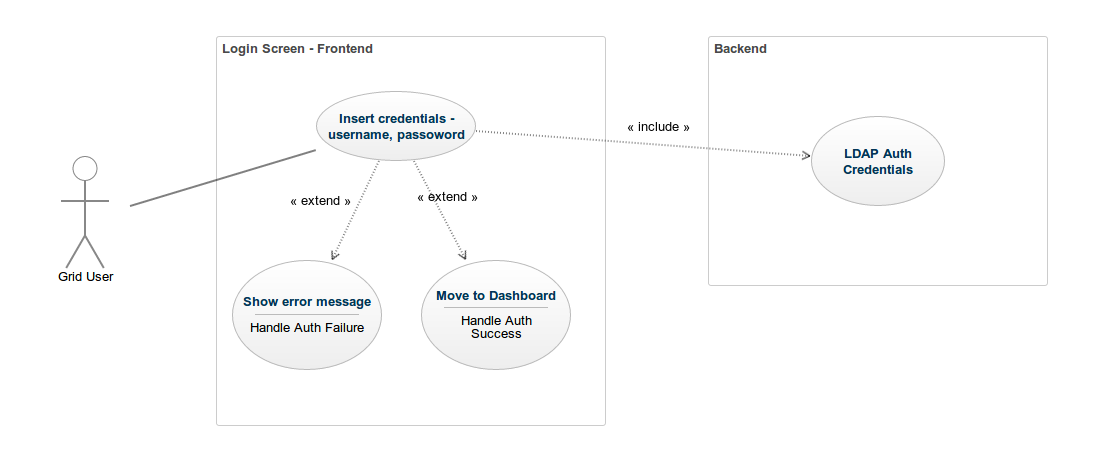
\includegraphics[width=16cm]{../images/login-use-case.png}
\centering
\end{figure}
\clearpage

\begin{figure}[t]
\caption{Screenshot - Login}
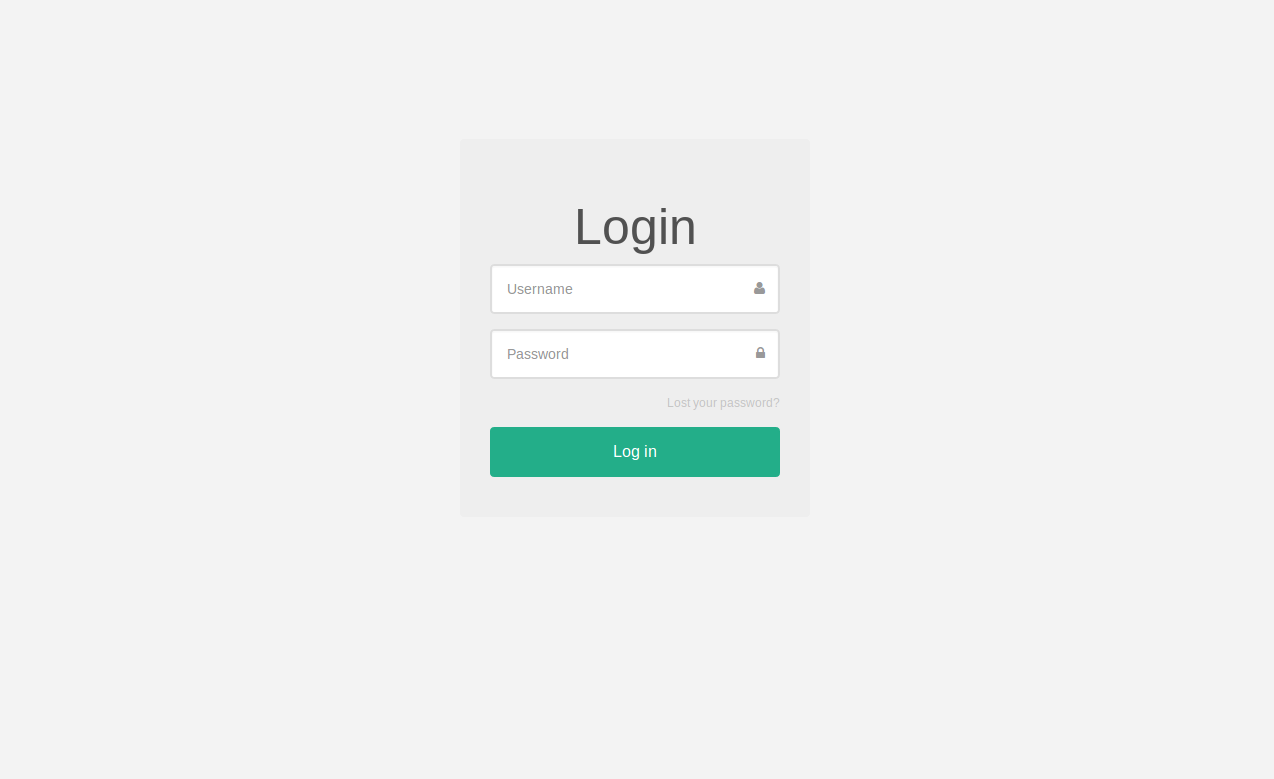
\includegraphics[width=16cm]{../images/login-screenshot.png}
\centering
\end{figure}
\clearpage

Μετά την επιτυχή επιβεβαίωση των στοιχείων, ο χρήστης μεταφέρετε στην κεντρική σελίδα της εφαρμογής.

\begin{figure}[t]
\caption{Screenshot - Home Page}
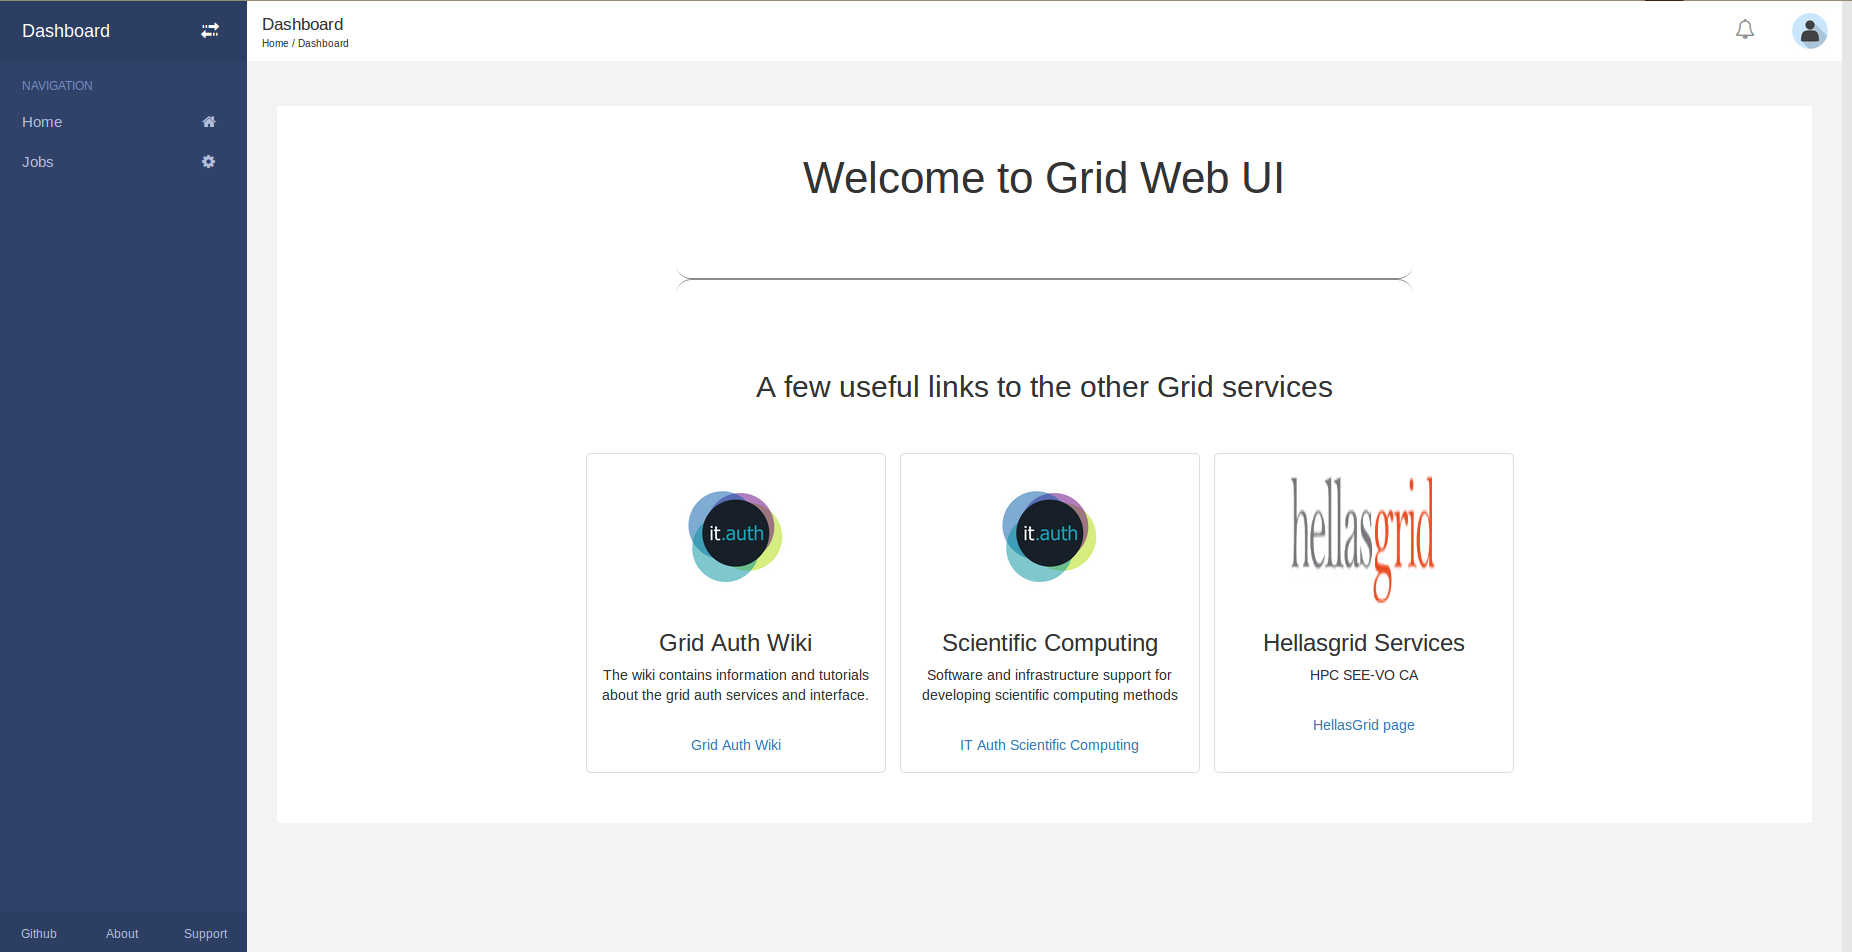
\includegraphics[width=16cm]{../images/home-page-screenshot.png}
\centering
\end{figure}
\clearpage


Αν τα στοιχεία του χρήστη είναι λανθασμένα θα του εμφανίσει ανάλογο μήνυμα και θα κοκκινίσει τα πεδία εισαγωγής.

\begin{figure}[t]
\caption{Screenshot - Invalid credentials}
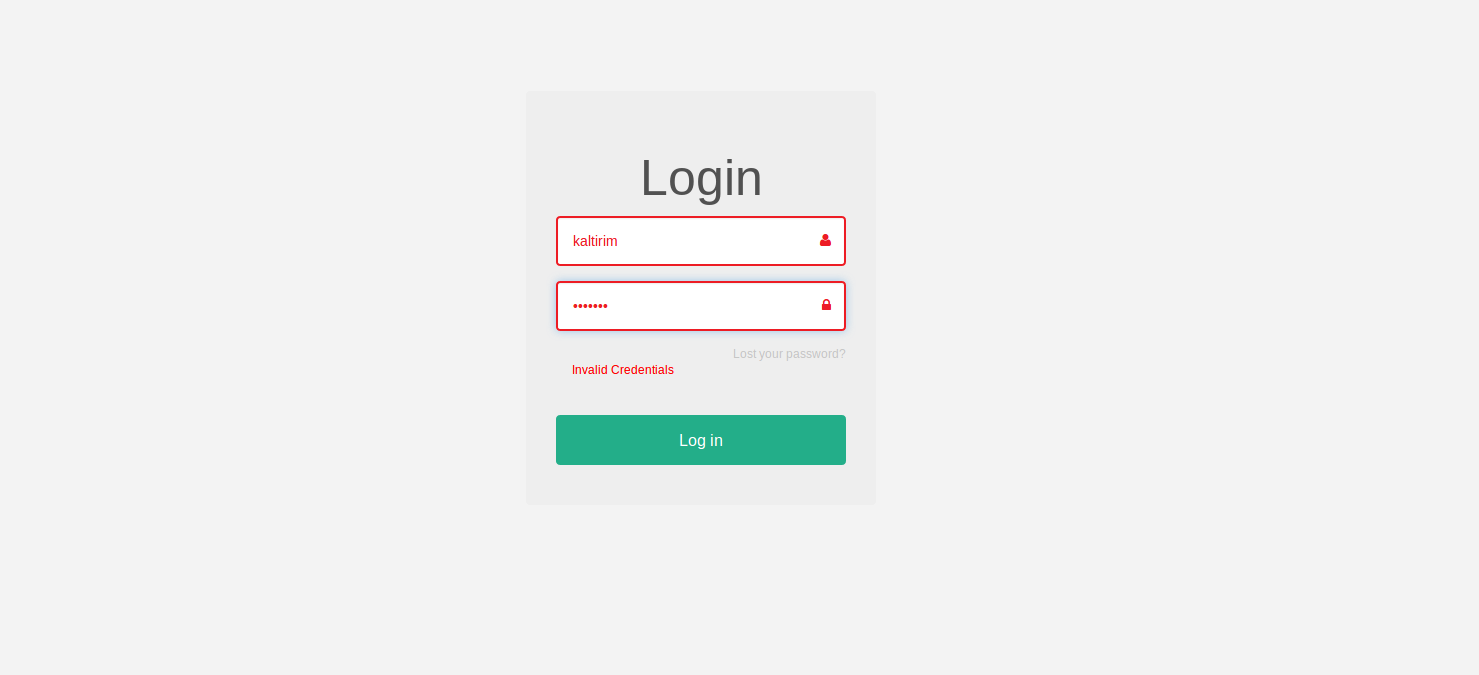
\includegraphics[width=16cm]{../images/invalid-credentials-screenshot.png}
\centering
\end{figure}
\clearpage

Σε περίπτωση που ο χρήστης έχει ξεχάσει τον κωδικό του, πατώντας τον σύνδεσμο \textit{Forgot you password} θα ανοίξει ένα καινούργιο παράθυρο στον \textit{browser} το οποίο αναλύει την διαδικασία ανάκτησης κωδικού, στο \textit{Grid Wiki}.

\begin{figure}[t]
\caption{Use case - Forgot password}
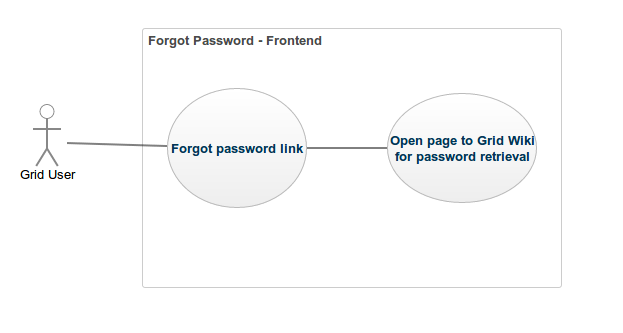
\includegraphics[width=16cm]{../images/forgot-password-case.png}
\centering
\end{figure}
\clearpage


\subsection{Έλεγχος εργασιών - View jobs}

Από το navigation menu στα δεξιά, της κάθε σελίδας, οι χρήστες μπορούν να μεταφερθούν στην σελίδα προβολής των εργασιών που έχουν υποβάλλει στη συστοιχία.

Αρχικά βλέπουν όλες τις εργασίες που έχουν υποβάλλει, και στη συνέχεια μπορούν να φιλτράρουν τις εργασίες για να δουν όποιες τους ενδιαφέρουν.
\newline
Το φιλτράρισμα μπορεί να γίνει με βάση τρεις διαφορετικούς παράγοντες. 
\newline
Την κατάσταση της εργασίας, η οποία μπορεί να είναι:
\begin{itemize}
\item Running - Η εργασία εκτελείται
\item Finished - Η εργασία έχει ολοκληρωθεί επιτυχώς
\item Stopped - Η εργασία έχει διακόψει την εκτέλεση της πριν ολοκληρωθεί
\end{itemize}
Την ημερομηνία υποβολής της εργασίας, από την πιο πρόσφατη έως την πιο παλιά και αντίστροφα.
\newline
Και τέλος αλφαβητικά με βάση το όνομα της εργασίας.
\newline
Τα φίλτρα μπορούν να χρησιμοποιηθούν και συνδυαστικά για να βγάλουν πιο συγκεκριμένα αποτελέσματα.

\begin{figure}[bp!]
\caption{Use case - View jobs}
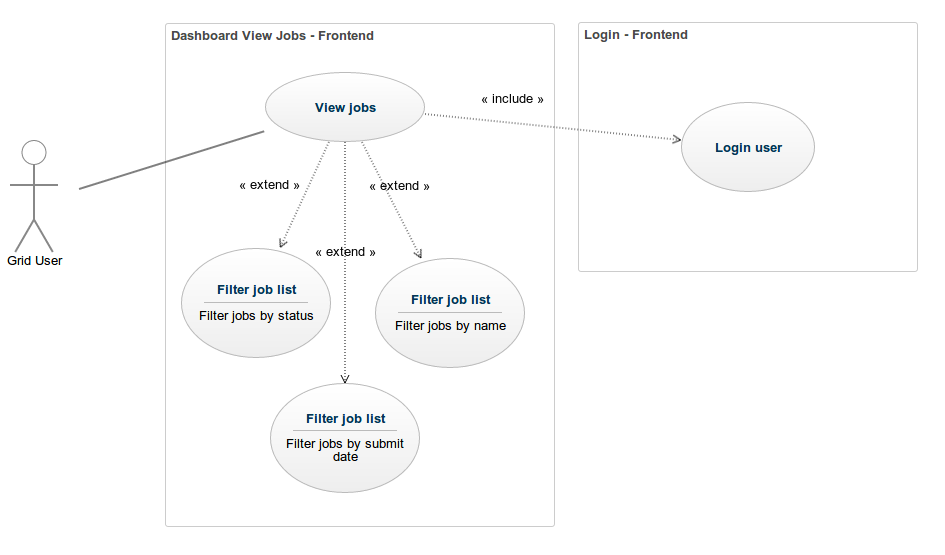
\includegraphics[width=16cm]{../images/view-jobs-case.png}
\centering
\end{figure}
\clearpage

\begin{figure}[bp!]
\caption{Screenshot - View Jobs}
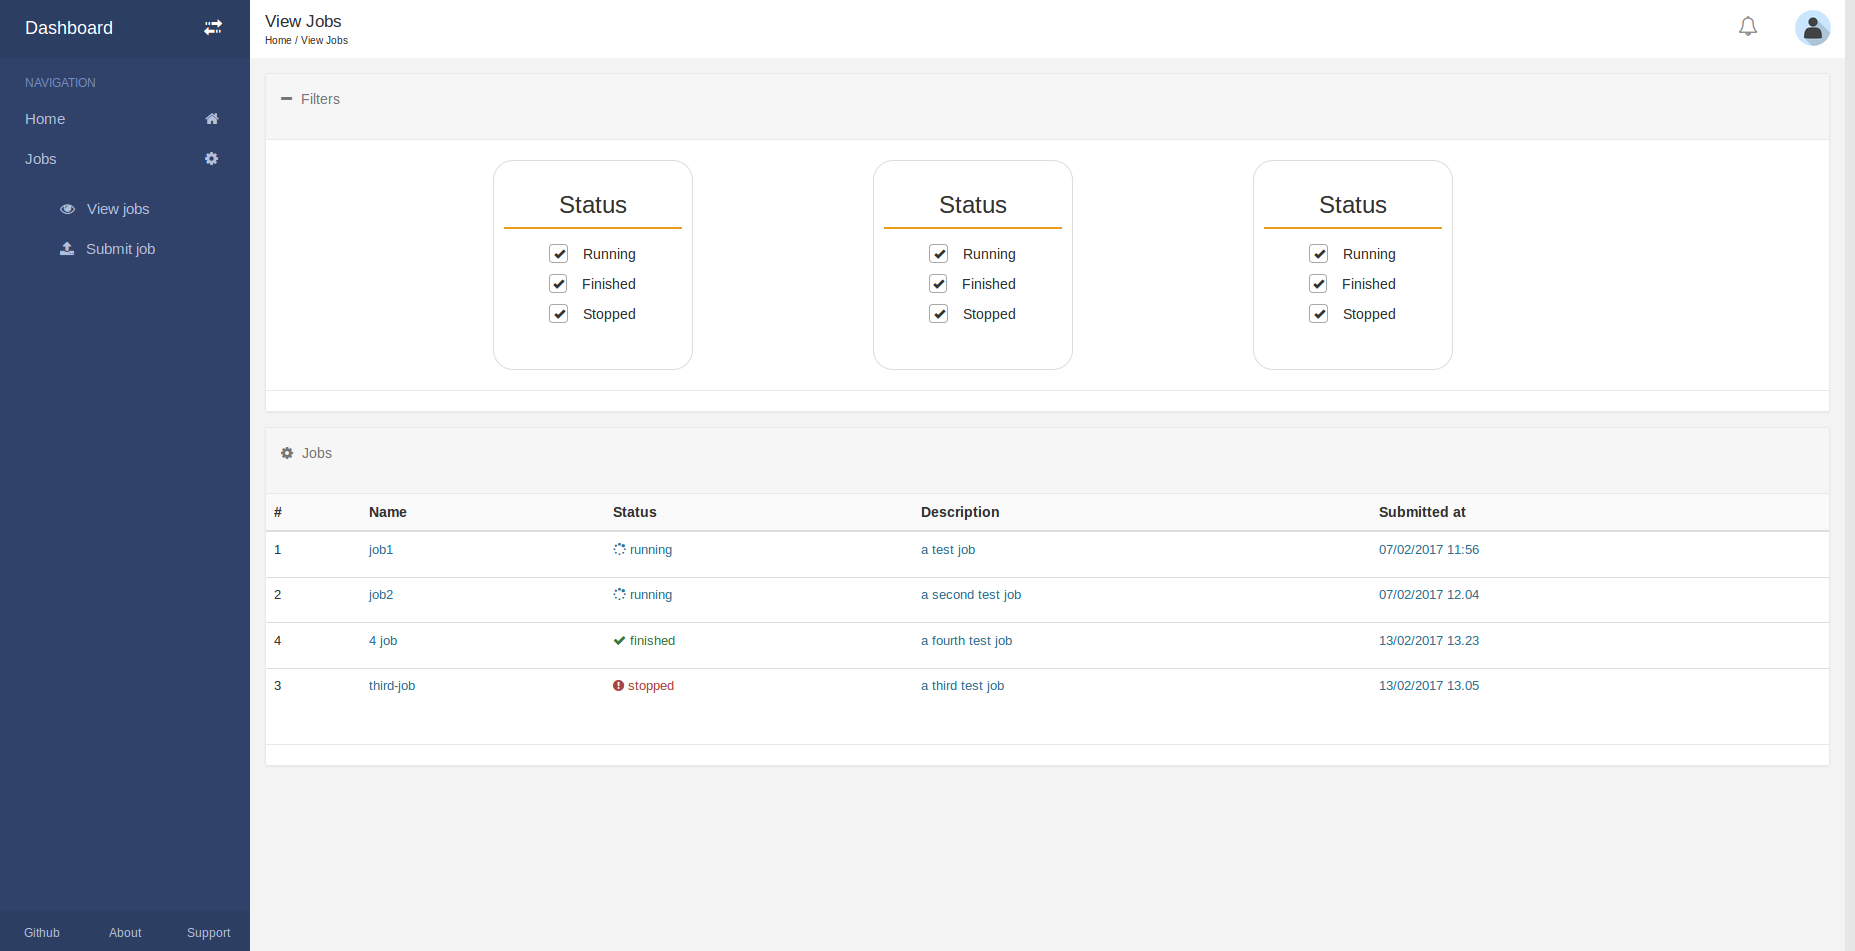
\includegraphics[width=16cm]{../images/view-jobs-screenshot.png}
\centering
\end{figure}
\clearpage


\subsection{Υποβολή νέας εργασίας - Submit job}

Από το αντίστοιχο μενού \textit{Navigation > Jobs} στα δεξιά της σελίδας, ο χρήστης μπορεί να επιλέξει το \textit{Submit job} για να υποβάλει μια νέα εργασία.  
\newline
Για να γίνει η υποβολή ο χρήστης θα πρέπει απαραίτητα να υποβάλει ένα εκτελέσιμο αρχείο. 
Επίσης μπορεί να προσθέσει αρχεία εισόδου για το πρόγραμμα ή να δώσει  \textit{file path} στο οποίο είναι αποθηκευμένα τα αρχεία εισόδου μέσα στην ιδρυματική συστοιχία. Τα αρχεία εισόδου που θα υποβάλει μέσα από το \textit{web application} μπορούν να είναι περισσότερα από ένα, καθώς και ολόκληροι φάκελοι. 
\newline

Στο κάτω μέρος της σελίδας μπορεί να δει ποια αρχεία έχει δηλώσει για υποβολή και να αφαιρέσει οποιοδήποτε δεν θέλει να συμπεριληφθούν στην εργασία.
\newline

\begin{figure}[bp!]
\caption{Use case - Create new job}
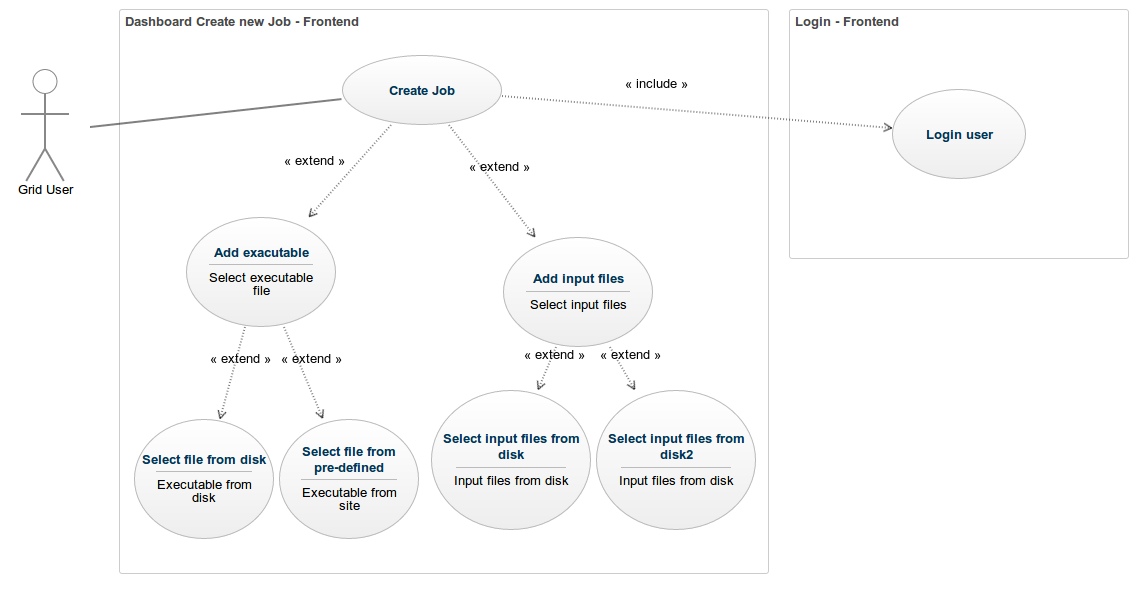
\includegraphics[width=16cm]{../images/create-job-case.png}
\centering
\end{figure}
\clearpage

\begin{figure}[bp!]
\caption{Screenshot - Create new job}
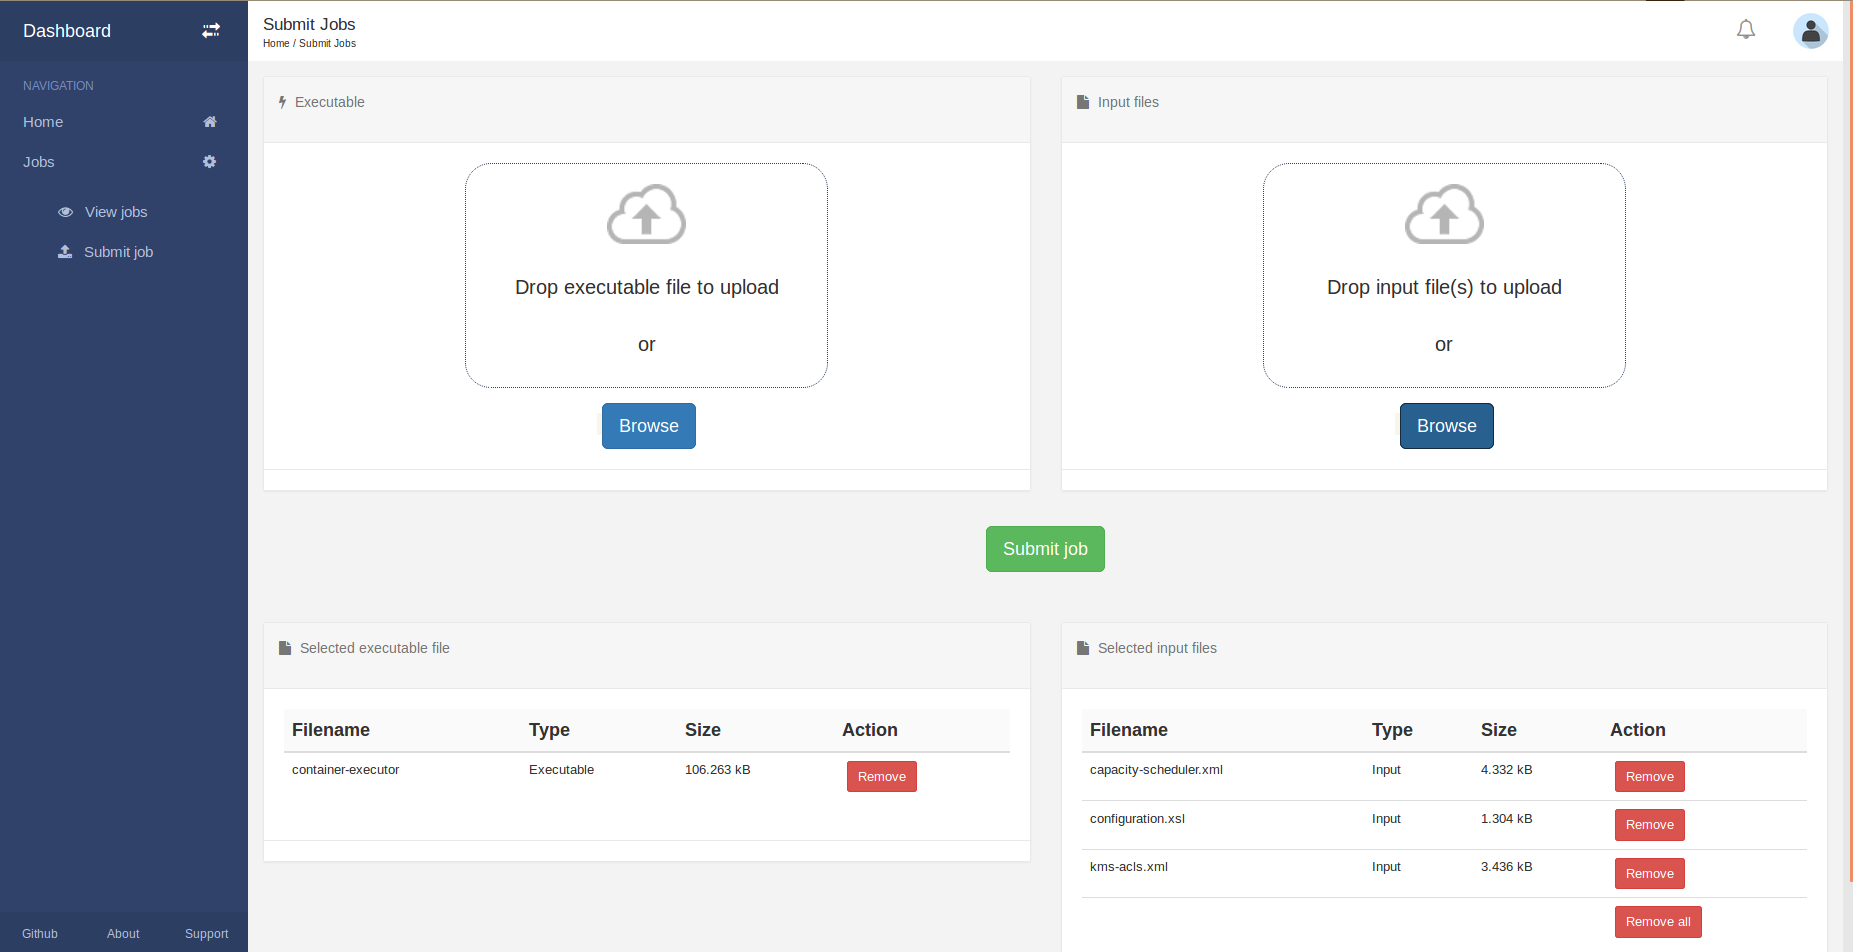
\includegraphics[width=16cm]{../images/submit-job-screenshot.png}
\centering
\end{figure}
\clearpage


Τέλος, αφού έχει υποβληθεί ένα εκτελέσιμο αρχείο, ο χρήστης μπορεί να υποβάλει την εργασία για εκτέλεση πατώντας το κουμπί \textit{submit}.

\begin{figure}[t]
\caption{Use case - Submit job}
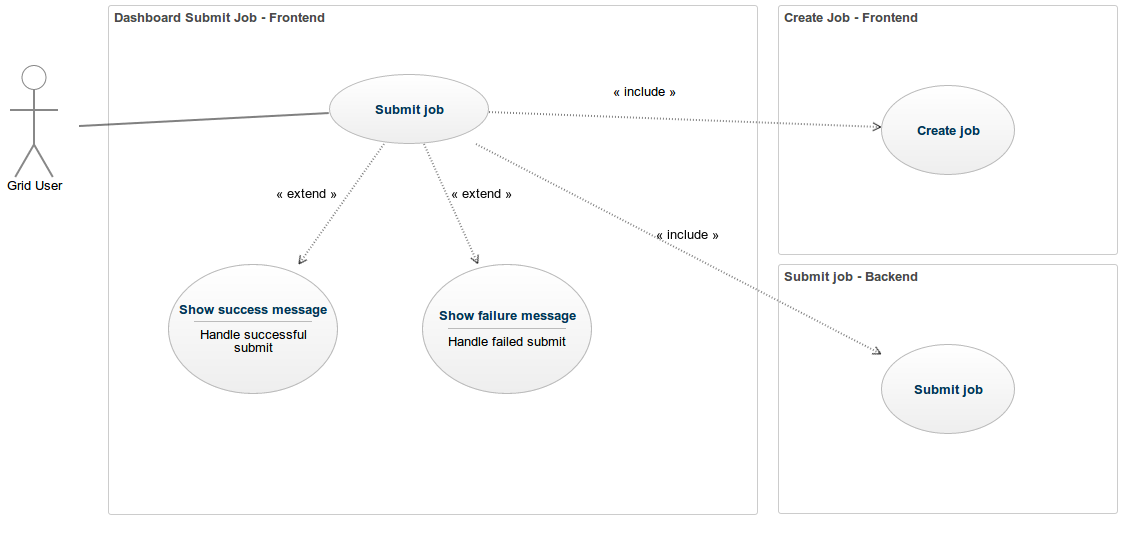
\includegraphics[width=16cm]{../images/submit-job-case.png}
\centering
\end{figure}
\clearpage




